\begin{figure}
  \centering
    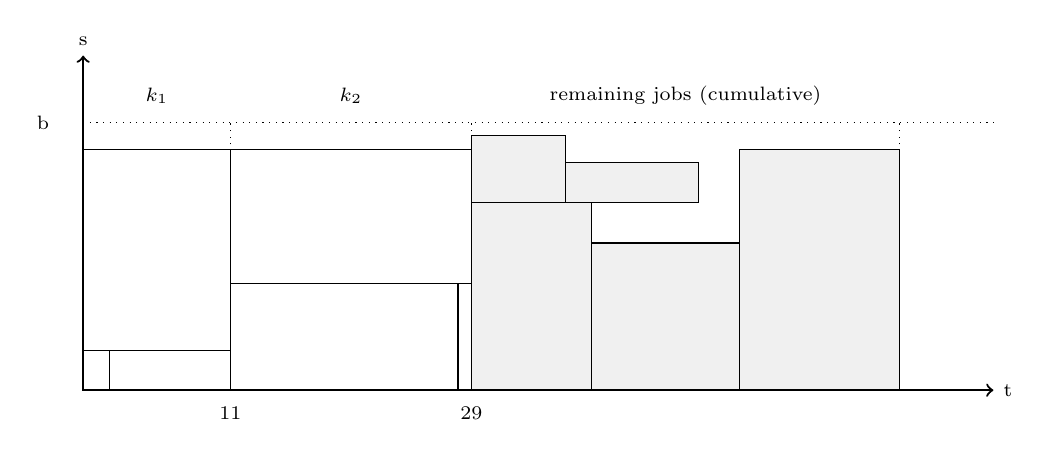
\begin{tikzpicture}[scale=0.17, font=\scriptsize]
            \draw[dotted] (0,20) -- (68,20);
      \node at (-3, 20) {{\sansitalicfont b }};
        \draw (0,0) rectangle (2,3) ;
        \draw (0,3) rectangle (11, 18); 
        \node at (5.5, 22) {$k_1$};
        \node at (11, -1.7) {\sansfont 11};
      \draw[dotted] (11,0) -- (11,20); 
        \draw (11,0) rectangle (28, 8) ;
        \draw (11,8) rectangle (29,18);
        \node at (20, 22) {$k_2$};
        \node at (29, -1.7) {\sansfont 29};
      \draw[dotted] (29,0) -- (29, 20);
        \draw[fill={rgb:black,1;white,16}](29,0) rectangle (38,14) ;
        \draw[fill={rgb:black,1;white,16}] (29,14) rectangle (36,19);
        \draw[fill={rgb:black,1;white,16}] (36,14) rectangle (46,17);
        \draw[fill={rgb:black,1;white,16}] (38,0) rectangle (49,11);
        \draw[fill={rgb:black,1;white,16}] (49,0) rectangle (61, 18);
\draw [<->,thick] (0,25) node (yaxis) [above] {\sansitalicfont s}
        |- (68,0) node (xaxis) [right] {\sansitalicfont t};

        \node at (45, 22) {remaining jobs (cumulative)};
      \draw[dotted] (61,0) -- (61, 20);

    \end{tikzpicture}
 \caption{Constructing the second batch. Remaining jobs are shaded.}\label{fig:decomp_tetris}
\end{figure}
